% Options for packages loaded elsewhere
\PassOptionsToPackage{unicode}{hyperref}
\PassOptionsToPackage{hyphens}{url}
\PassOptionsToPackage{dvipsnames,svgnames,x11names}{xcolor}
%
\documentclass[
  letterpaper,
  DIV=11,
  numbers=noendperiod]{scrartcl}

\usepackage{amsmath,amssymb}
\usepackage{iftex}
\ifPDFTeX
  \usepackage[T1]{fontenc}
  \usepackage[utf8]{inputenc}
  \usepackage{textcomp} % provide euro and other symbols
\else % if luatex or xetex
  \usepackage{unicode-math}
  \defaultfontfeatures{Scale=MatchLowercase}
  \defaultfontfeatures[\rmfamily]{Ligatures=TeX,Scale=1}
\fi
\usepackage{lmodern}
\ifPDFTeX\else  
    % xetex/luatex font selection
\fi
% Use upquote if available, for straight quotes in verbatim environments
\IfFileExists{upquote.sty}{\usepackage{upquote}}{}
\IfFileExists{microtype.sty}{% use microtype if available
  \usepackage[]{microtype}
  \UseMicrotypeSet[protrusion]{basicmath} % disable protrusion for tt fonts
}{}
\makeatletter
\@ifundefined{KOMAClassName}{% if non-KOMA class
  \IfFileExists{parskip.sty}{%
    \usepackage{parskip}
  }{% else
    \setlength{\parindent}{0pt}
    \setlength{\parskip}{6pt plus 2pt minus 1pt}}
}{% if KOMA class
  \KOMAoptions{parskip=half}}
\makeatother
\usepackage{xcolor}
\setlength{\emergencystretch}{3em} % prevent overfull lines
\setcounter{secnumdepth}{5}
% Make \paragraph and \subparagraph free-standing
\makeatletter
\ifx\paragraph\undefined\else
  \let\oldparagraph\paragraph
  \renewcommand{\paragraph}{
    \@ifstar
      \xxxParagraphStar
      \xxxParagraphNoStar
  }
  \newcommand{\xxxParagraphStar}[1]{\oldparagraph*{#1}\mbox{}}
  \newcommand{\xxxParagraphNoStar}[1]{\oldparagraph{#1}\mbox{}}
\fi
\ifx\subparagraph\undefined\else
  \let\oldsubparagraph\subparagraph
  \renewcommand{\subparagraph}{
    \@ifstar
      \xxxSubParagraphStar
      \xxxSubParagraphNoStar
  }
  \newcommand{\xxxSubParagraphStar}[1]{\oldsubparagraph*{#1}\mbox{}}
  \newcommand{\xxxSubParagraphNoStar}[1]{\oldsubparagraph{#1}\mbox{}}
\fi
\makeatother

\usepackage{color}
\usepackage{fancyvrb}
\newcommand{\VerbBar}{|}
\newcommand{\VERB}{\Verb[commandchars=\\\{\}]}
\DefineVerbatimEnvironment{Highlighting}{Verbatim}{commandchars=\\\{\}}
% Add ',fontsize=\small' for more characters per line
\usepackage{framed}
\definecolor{shadecolor}{RGB}{241,243,245}
\newenvironment{Shaded}{\begin{snugshade}}{\end{snugshade}}
\newcommand{\AlertTok}[1]{\textcolor[rgb]{0.68,0.00,0.00}{#1}}
\newcommand{\AnnotationTok}[1]{\textcolor[rgb]{0.37,0.37,0.37}{#1}}
\newcommand{\AttributeTok}[1]{\textcolor[rgb]{0.40,0.45,0.13}{#1}}
\newcommand{\BaseNTok}[1]{\textcolor[rgb]{0.68,0.00,0.00}{#1}}
\newcommand{\BuiltInTok}[1]{\textcolor[rgb]{0.00,0.23,0.31}{#1}}
\newcommand{\CharTok}[1]{\textcolor[rgb]{0.13,0.47,0.30}{#1}}
\newcommand{\CommentTok}[1]{\textcolor[rgb]{0.37,0.37,0.37}{#1}}
\newcommand{\CommentVarTok}[1]{\textcolor[rgb]{0.37,0.37,0.37}{\textit{#1}}}
\newcommand{\ConstantTok}[1]{\textcolor[rgb]{0.56,0.35,0.01}{#1}}
\newcommand{\ControlFlowTok}[1]{\textcolor[rgb]{0.00,0.23,0.31}{\textbf{#1}}}
\newcommand{\DataTypeTok}[1]{\textcolor[rgb]{0.68,0.00,0.00}{#1}}
\newcommand{\DecValTok}[1]{\textcolor[rgb]{0.68,0.00,0.00}{#1}}
\newcommand{\DocumentationTok}[1]{\textcolor[rgb]{0.37,0.37,0.37}{\textit{#1}}}
\newcommand{\ErrorTok}[1]{\textcolor[rgb]{0.68,0.00,0.00}{#1}}
\newcommand{\ExtensionTok}[1]{\textcolor[rgb]{0.00,0.23,0.31}{#1}}
\newcommand{\FloatTok}[1]{\textcolor[rgb]{0.68,0.00,0.00}{#1}}
\newcommand{\FunctionTok}[1]{\textcolor[rgb]{0.28,0.35,0.67}{#1}}
\newcommand{\ImportTok}[1]{\textcolor[rgb]{0.00,0.46,0.62}{#1}}
\newcommand{\InformationTok}[1]{\textcolor[rgb]{0.37,0.37,0.37}{#1}}
\newcommand{\KeywordTok}[1]{\textcolor[rgb]{0.00,0.23,0.31}{\textbf{#1}}}
\newcommand{\NormalTok}[1]{\textcolor[rgb]{0.00,0.23,0.31}{#1}}
\newcommand{\OperatorTok}[1]{\textcolor[rgb]{0.37,0.37,0.37}{#1}}
\newcommand{\OtherTok}[1]{\textcolor[rgb]{0.00,0.23,0.31}{#1}}
\newcommand{\PreprocessorTok}[1]{\textcolor[rgb]{0.68,0.00,0.00}{#1}}
\newcommand{\RegionMarkerTok}[1]{\textcolor[rgb]{0.00,0.23,0.31}{#1}}
\newcommand{\SpecialCharTok}[1]{\textcolor[rgb]{0.37,0.37,0.37}{#1}}
\newcommand{\SpecialStringTok}[1]{\textcolor[rgb]{0.13,0.47,0.30}{#1}}
\newcommand{\StringTok}[1]{\textcolor[rgb]{0.13,0.47,0.30}{#1}}
\newcommand{\VariableTok}[1]{\textcolor[rgb]{0.07,0.07,0.07}{#1}}
\newcommand{\VerbatimStringTok}[1]{\textcolor[rgb]{0.13,0.47,0.30}{#1}}
\newcommand{\WarningTok}[1]{\textcolor[rgb]{0.37,0.37,0.37}{\textit{#1}}}

\providecommand{\tightlist}{%
  \setlength{\itemsep}{0pt}\setlength{\parskip}{0pt}}\usepackage{longtable,booktabs,array}
\usepackage{calc} % for calculating minipage widths
% Correct order of tables after \paragraph or \subparagraph
\usepackage{etoolbox}
\makeatletter
\patchcmd\longtable{\par}{\if@noskipsec\mbox{}\fi\par}{}{}
\makeatother
% Allow footnotes in longtable head/foot
\IfFileExists{footnotehyper.sty}{\usepackage{footnotehyper}}{\usepackage{footnote}}
\makesavenoteenv{longtable}
\usepackage{graphicx}
\makeatletter
\def\maxwidth{\ifdim\Gin@nat@width>\linewidth\linewidth\else\Gin@nat@width\fi}
\def\maxheight{\ifdim\Gin@nat@height>\textheight\textheight\else\Gin@nat@height\fi}
\makeatother
% Scale images if necessary, so that they will not overflow the page
% margins by default, and it is still possible to overwrite the defaults
% using explicit options in \includegraphics[width, height, ...]{}
\setkeys{Gin}{width=\maxwidth,height=\maxheight,keepaspectratio}
% Set default figure placement to htbp
\makeatletter
\def\fps@figure{htbp}
\makeatother

\KOMAoption{captions}{tableheading}
\makeatletter
\@ifpackageloaded{caption}{}{\usepackage{caption}}
\AtBeginDocument{%
\ifdefined\contentsname
  \renewcommand*\contentsname{Table of contents}
\else
  \newcommand\contentsname{Table of contents}
\fi
\ifdefined\listfigurename
  \renewcommand*\listfigurename{List of Figures}
\else
  \newcommand\listfigurename{List of Figures}
\fi
\ifdefined\listtablename
  \renewcommand*\listtablename{List of Tables}
\else
  \newcommand\listtablename{List of Tables}
\fi
\ifdefined\figurename
  \renewcommand*\figurename{Figure}
\else
  \newcommand\figurename{Figure}
\fi
\ifdefined\tablename
  \renewcommand*\tablename{Table}
\else
  \newcommand\tablename{Table}
\fi
}
\@ifpackageloaded{float}{}{\usepackage{float}}
\floatstyle{ruled}
\@ifundefined{c@chapter}{\newfloat{codelisting}{h}{lop}}{\newfloat{codelisting}{h}{lop}[chapter]}
\floatname{codelisting}{Listing}
\newcommand*\listoflistings{\listof{codelisting}{List of Listings}}
\makeatother
\makeatletter
\makeatother
\makeatletter
\@ifpackageloaded{caption}{}{\usepackage{caption}}
\@ifpackageloaded{subcaption}{}{\usepackage{subcaption}}
\makeatother

\ifLuaTeX
  \usepackage{selnolig}  % disable illegal ligatures
\fi
\usepackage{bookmark}

\IfFileExists{xurl.sty}{\usepackage{xurl}}{} % add URL line breaks if available
\urlstyle{same} % disable monospaced font for URLs
\hypersetup{
  pdftitle={Social Network - Assignment \#1},
  pdfauthor={Aurora Sterpellone - Gür Piren},
  colorlinks=true,
  linkcolor={blue},
  filecolor={Maroon},
  citecolor={Blue},
  urlcolor={Blue},
  pdfcreator={LaTeX via pandoc}}


\title{Social Network - Assignment \#1}
\author{Aurora Sterpellone - Gür Piren}
\date{2025-04-22}

\begin{document}
\maketitle

\renewcommand*\contentsname{Table of contents}
{
\hypersetup{linkcolor=}
\setcounter{tocdepth}{3}
\tableofcontents
}

\section{Introduction}\label{introduction}

Through this file, we will reveal the number and nature of the
partnerships between heroes, villains, and neutral characters across the
Marvel Universe. While doing so, we will try to answer a number of
questions that were raised as part of the first homework assignment for
the Social Network Analysis.

\subsection{Acknowledgements}\label{acknowledgements}

The AI was utilized as a complementary tool to have a better grasp of
the concepts and questions across the file. Our interpretations of some
of the results were secured through AI perspective. Although we sticked
to the in-class exercises and files, some of the plots were created
using the AI support.

\subsection{Libraries}\label{libraries}

\begin{Shaded}
\begin{Highlighting}[]
\FunctionTok{library}\NormalTok{(igraph)}
\FunctionTok{library}\NormalTok{(stringr)}
\FunctionTok{library}\NormalTok{(dplyr)}
\FunctionTok{library}\NormalTok{(ggraph) }\CommentTok{\# ultimately, might not use it. check at the end}
\FunctionTok{library}\NormalTok{(tidygraph) }\CommentTok{\# ultimately, might not use it. check at the end}
\FunctionTok{library}\NormalTok{(ggrepel)}
\FunctionTok{library}\NormalTok{(extrafont)}
\FunctionTok{library}\NormalTok{(tibble)}
\FunctionTok{library}\NormalTok{(fmsb)}
\FunctionTok{library}\NormalTok{(GGally)}
\FunctionTok{library}\NormalTok{(tidyr)}
\end{Highlighting}
\end{Shaded}

\section{Questions}\label{questions}

\subsection{Choose a network dataset}\label{choose-a-network-dataset}

Marvel character partnerships, 2018. The dataset can be accessed through
this \href{https://networks.skewed.de/net/marvel_partnerships}{link}

\subsection{Indicate the number of nodes. It should be larger than 300
but smaller than
10000.}\label{indicate-the-number-of-nodes.-it-should-be-larger-than-300-but-smaller-than-10000.}

The number of nodes is 350.

\begin{Shaded}
\begin{Highlighting}[]
\FunctionTok{load}\NormalTok{(}\StringTok{"marvel\_network.rda"}\NormalTok{)}

\CommentTok{\# for the number of nodes}
\NormalTok{num\_nodes }\OtherTok{\textless{}{-}} \FunctionTok{vcount}\NormalTok{(marvel\_network)}

\FunctionTok{cat}\NormalTok{(}\StringTok{"Number of nodes:"}\NormalTok{, num\_nodes)}
\end{Highlighting}
\end{Shaded}

\begin{verbatim}
Number of nodes: 350
\end{verbatim}

\subsection{Import that data and create a graph using
R.}\label{import-that-data-and-create-a-graph-using-r.}

Reading the data first. The original network will be plotted after a
quick data description and cleaning process.

\begin{Shaded}
\begin{Highlighting}[]
\NormalTok{marvel\_nodes }\OtherTok{\textless{}{-}} \FunctionTok{read.csv}\NormalTok{(}\StringTok{"data/nodes.csv"}\NormalTok{, }\AttributeTok{stringsAsFactors =} \ConstantTok{FALSE}\NormalTok{,}
                         \AttributeTok{quote =} \StringTok{"}\SpecialCharTok{\textbackslash{}"}\StringTok{"}\NormalTok{, }\AttributeTok{fill =} \ConstantTok{TRUE}\NormalTok{)}

\NormalTok{marvel\_links }\OtherTok{\textless{}{-}} \FunctionTok{read.csv}\NormalTok{(}\StringTok{"data/edges.csv"}\NormalTok{, }\AttributeTok{stringsAsFactors =} \ConstantTok{FALSE}\NormalTok{)}
\end{Highlighting}
\end{Shaded}

\subsubsection{Data description}\label{data-description}

Initially, we have two datasets separately for nodes and links. Later
on, they will be merged.

\begin{enumerate}
\def\labelenumi{\arabic{enumi}.}
\tightlist
\item
  The dataset for the nodes includes the following variables:
\end{enumerate}

\textbf{id:} The index number of the character in the network.

\textbf{character\_name:} The name of the character, which could be a
hero, villain, or neutral character.

\textbf{group:} Indicates the category of the character (e.g., hero,
villain, or neutral).

\textbf{size:} Represents the number of partnerships the character has
within the network.

\textbf{x:} The X-coordinate that positions the character in the network
layout.

\textbf{y:} The Y-coordinate that positions the character in the network
layout.

\begin{enumerate}
\def\labelenumi{\arabic{enumi}.}
\setcounter{enumi}{1}
\tightlist
\item
  The dataset for the links, on the other hand, incorporates the
  following variables:
\end{enumerate}

\textbf{source:} This column represents the starting character in a
partnership (the character initiating or belonging to the partnership).

\textbf{target:} This column indicates the partner in the relationship
with the source character.

\subsubsection{Data cleaning}\label{data-cleaning}

Let's read both datasets, treating text as characters (not factors), and
ensuring quotes and missing data are handled properly.

\begin{Shaded}
\begin{Highlighting}[]
\CommentTok{\# to get proper x and y coordinates}

\NormalTok{marvel\_nodes}\SpecialCharTok{$}\NormalTok{pos\_x }\OtherTok{\textless{}{-}} \FunctionTok{as.numeric}\NormalTok{(}\FunctionTok{str\_extract}\NormalTok{(marvel\_nodes}\SpecialCharTok{$}\NormalTok{X\_pos,}
                                             \StringTok{"{-}?}\SpecialCharTok{\textbackslash{}\textbackslash{}}\StringTok{d+}\SpecialCharTok{\textbackslash{}\textbackslash{}}\StringTok{.}\SpecialCharTok{\textbackslash{}\textbackslash{}}\StringTok{d+"}\NormalTok{))}
\NormalTok{marvel\_nodes}\SpecialCharTok{$}\NormalTok{pos\_y }\OtherTok{\textless{}{-}} \FunctionTok{as.numeric}\NormalTok{(}\FunctionTok{str\_extract\_all}\NormalTok{(marvel\_nodes}\SpecialCharTok{$}\NormalTok{X\_pos,}
                                                 \StringTok{"{-}?}\SpecialCharTok{\textbackslash{}\textbackslash{}}\StringTok{d+}\SpecialCharTok{\textbackslash{}\textbackslash{}}\StringTok{.}\SpecialCharTok{\textbackslash{}\textbackslash{}}\StringTok{d+"}\NormalTok{) }\SpecialCharTok{\%\textgreater{}\%} 
                                   \FunctionTok{sapply}\NormalTok{(}\StringTok{\textasciigrave{}}\AttributeTok{[}\StringTok{\textasciigrave{}}\NormalTok{, }\DecValTok{2}\NormalTok{))}

\CommentTok{\# we don\textquotesingle{}t need the X\_pos anymore}
\NormalTok{marvel\_nodes}\SpecialCharTok{$}\NormalTok{X\_pos }\OtherTok{\textless{}{-}} \ConstantTok{NULL}
\end{Highlighting}
\end{Shaded}

\subsubsection{Renaming columns}\label{renaming-columns}

To improve readability, we will rename certain columns in both datasets.
After that, we will remove any alternative names or descriptions that
appear in parentheses following a character's name.

\begin{Shaded}
\begin{Highlighting}[]
\NormalTok{marvel\_nodes }\OtherTok{\textless{}{-}}\NormalTok{ marvel\_nodes }\SpecialCharTok{|\textgreater{}} 
  \FunctionTok{rename}\NormalTok{(}\AttributeTok{id =}\NormalTok{ X..index,}
         \AttributeTok{character\_name =}\NormalTok{ id,}
         \AttributeTok{x =}\NormalTok{ pos\_x,}
         \AttributeTok{y =}\NormalTok{ pos\_y) }\SpecialCharTok{|\textgreater{}} 
  \FunctionTok{mutate}\NormalTok{(}\AttributeTok{id =}\NormalTok{ id }\SpecialCharTok{+} \DecValTok{1}\NormalTok{) }\CommentTok{\# for best indexing practice}

\NormalTok{marvel\_links }\OtherTok{\textless{}{-}}\NormalTok{ marvel\_links }\SpecialCharTok{|\textgreater{}} 
  \FunctionTok{rename}\NormalTok{(}\AttributeTok{source =}\NormalTok{ X..source,}
         \AttributeTok{target =}\NormalTok{ target)}

\NormalTok{marvel\_links }\OtherTok{\textless{}{-}}\NormalTok{ marvel\_links }\SpecialCharTok{|\textgreater{}} 
  \FunctionTok{mutate}\NormalTok{(}\AttributeTok{source =}\NormalTok{ source }\SpecialCharTok{+} \DecValTok{1}\NormalTok{,}
         \AttributeTok{target =}\NormalTok{ target }\SpecialCharTok{+} \DecValTok{1}\NormalTok{)}

\CommentTok{\# let\textquotesingle{}s get rid of anything that is in parentheses in the character\_name columns}
\NormalTok{marvel\_nodes}\SpecialCharTok{$}\NormalTok{character\_name }\OtherTok{\textless{}{-}} \FunctionTok{gsub}\NormalTok{(}\StringTok{" }\SpecialCharTok{\textbackslash{}\textbackslash{}}\StringTok{(.*?}\SpecialCharTok{\textbackslash{}\textbackslash{}}\StringTok{)"}\NormalTok{, }\StringTok{""}\NormalTok{,}
\NormalTok{                                    marvel\_nodes}\SpecialCharTok{$}\NormalTok{character\_name)}
\end{Highlighting}
\end{Shaded}

\subsubsection{Plot}\label{plot}

Plotting the network, without distinguishing between heroes, villains,
and neutral characters.

\begin{Shaded}
\begin{Highlighting}[]
\NormalTok{marvel\_network }\OtherTok{\textless{}{-}} \FunctionTok{graph\_from\_data\_frame}\NormalTok{(}\AttributeTok{d =}\NormalTok{ marvel\_links,}
                                        \AttributeTok{vertices =}\NormalTok{ marvel\_nodes,}
                                        \AttributeTok{directed =} \ConstantTok{FALSE}\NormalTok{)}

\NormalTok{etiqueta }\OtherTok{\textless{}{-}} \FunctionTok{ifelse}\NormalTok{(}\FunctionTok{degree}\NormalTok{(marvel\_network) }\SpecialCharTok{\textgreater{}} \DecValTok{5}\NormalTok{,}
                   \FunctionTok{V}\NormalTok{(marvel\_network)}\SpecialCharTok{$}\NormalTok{character\_name, }\StringTok{""}\NormalTok{)}

\CommentTok{\# Plot the network}
\FunctionTok{plot}\NormalTok{(marvel\_network,}
     \AttributeTok{vertex.size =} \FunctionTok{degree}\NormalTok{(marvel\_network),  }\CommentTok{\# Node size by degree}
     \AttributeTok{edge.width =} \DecValTok{1}\NormalTok{,  }\CommentTok{\# No edge value attribute, set to constant}
     \AttributeTok{vertex.color =} \StringTok{"lightblue"}\NormalTok{,  }\CommentTok{\# No colour attribute, use a constant color}
     \AttributeTok{vertex.label =}\NormalTok{ etiqueta,}
     \AttributeTok{vertex.label.family =} \StringTok{"Marvel"}\NormalTok{,  }\CommentTok{\# Use your font}
     \AttributeTok{vertex.label.dist =} \DecValTok{1}\NormalTok{,}
     \AttributeTok{vertex.label.cex =} \FloatTok{1.0}\NormalTok{)}
\end{Highlighting}
\end{Shaded}

\includegraphics{Social_Network_1st_Assignment_files/figure-pdf/marvel-network-plot-1.pdf}

\begin{Shaded}
\begin{Highlighting}[]
\FunctionTok{save}\NormalTok{(marvel\_network, }\AttributeTok{file =} \StringTok{"marvel\_network.rda"}\NormalTok{)}
\end{Highlighting}
\end{Shaded}

Let's work on a cleaner plot, ideally we wanted to plot it with those
characters that has the biggest sizes (number of partnerships) only, but
we were not able to position the node labels clearly.

For the font of use:

\begin{Shaded}
\begin{Highlighting}[]
\FunctionTok{font\_import}\NormalTok{(}\AttributeTok{pattern =} \StringTok{"Marvel"}\NormalTok{) }
\end{Highlighting}
\end{Shaded}

\begin{verbatim}
Importing fonts may take a few minutes, depending on the number of fonts and the speed of the system.
Continue? [y/n] 
\end{verbatim}

\begin{Shaded}
\begin{Highlighting}[]
\FunctionTok{loadfonts}\NormalTok{() }

\CommentTok{\# setting font globally}
\FunctionTok{par}\NormalTok{(}\AttributeTok{family =} \StringTok{"Marvel"}\NormalTok{)}
\end{Highlighting}
\end{Shaded}

For the colours, we created a unique palette using the colours for the
main Marvel superheroes:

\begin{figure}[H]

{\centering 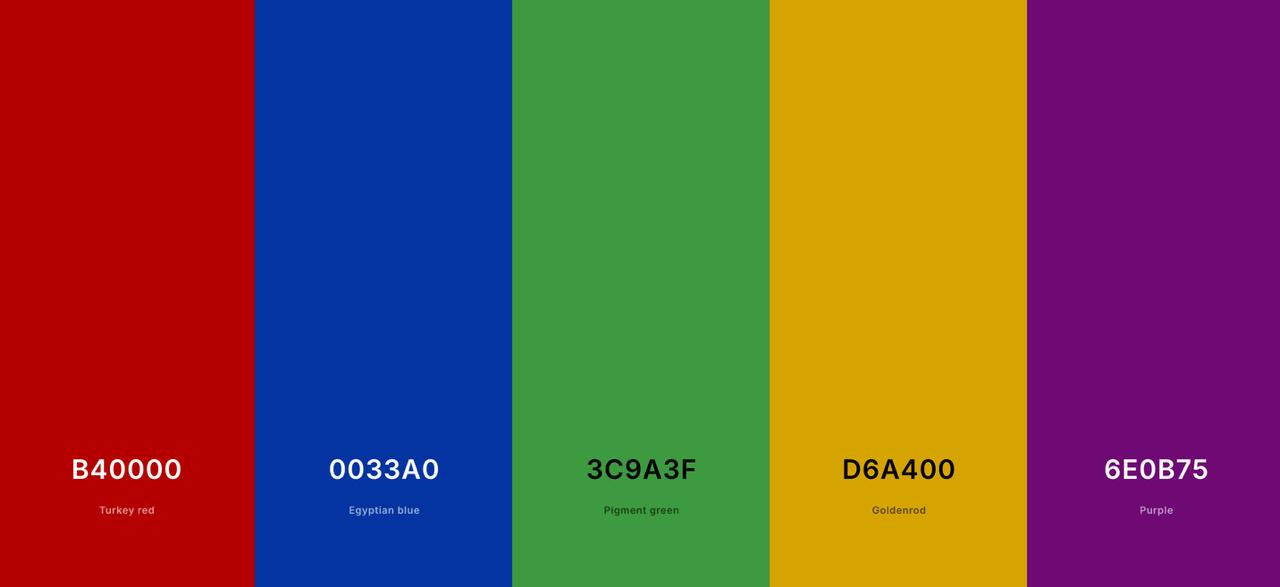
\includegraphics{./marvel_palette.jpeg}

}

\caption{Marvel Color Palette}

\end{figure}%

\begin{enumerate}
\def\labelenumi{\arabic{enumi}.}
\item
  Iron Man Red -- \#B40000
\item
  Captain America Blue -- \#0033A0
\item
  Hulk Green -- \#3C9A3F
\item
  Thor Gold -- \#D6A400
\item
  Loki Purple -- \#6E0B75
\end{enumerate}

\begin{Shaded}
\begin{Highlighting}[]
\CommentTok{\# defining a color for each group {-} heroes \textquotesingle{}0\textquotesingle{}, villains \textquotesingle{}1\textquotesingle{}, and neither \textquotesingle{}2\textquotesingle{}}

\NormalTok{group\_colors }\OtherTok{\textless{}{-}} \FunctionTok{c}\NormalTok{(}\StringTok{"0"} \OtherTok{=} \StringTok{"\#B40000"}\NormalTok{, }\StringTok{"1"} \OtherTok{=} \StringTok{"\#0033A0"}\NormalTok{, }\StringTok{"2"} \OtherTok{=} \StringTok{"\#3C9A3F"}\NormalTok{)}
\end{Highlighting}
\end{Shaded}

\begin{Shaded}
\begin{Highlighting}[]
\FunctionTok{V}\NormalTok{(marvel\_network)}\SpecialCharTok{$}\NormalTok{group }\OtherTok{\textless{}{-}}\NormalTok{ marvel\_nodes}\SpecialCharTok{$}\NormalTok{group}

\FunctionTok{plot}\NormalTok{(marvel\_network, }
     \AttributeTok{vertex.label =} \ConstantTok{NA}\NormalTok{,                      }
     \AttributeTok{vertex.size =} \DecValTok{5}\NormalTok{,                        }
     \AttributeTok{edge.color =} \StringTok{"gray15"}\NormalTok{,                  }
     \AttributeTok{vertex.color =}\NormalTok{ group\_colors[}\FunctionTok{as.character}\NormalTok{(}\FunctionTok{V}\NormalTok{(marvel\_network)}\SpecialCharTok{$}\NormalTok{group)], }
     \AttributeTok{layout =} \FunctionTok{cbind}\NormalTok{(}\FunctionTok{V}\NormalTok{(marvel\_network)}\SpecialCharTok{$}\NormalTok{x, }\FunctionTok{V}\NormalTok{(marvel\_network)}\SpecialCharTok{$}\NormalTok{y))  }

\FunctionTok{title}\NormalTok{(}\StringTok{"Marvel Partnerships Network"}\NormalTok{, }\AttributeTok{cex.main =} \FloatTok{1.2}\NormalTok{)}

\CommentTok{\# for the legend}
\FunctionTok{legend}\NormalTok{(}\StringTok{"topleft"}\NormalTok{, }
       \AttributeTok{legend =} \FunctionTok{c}\NormalTok{(}\StringTok{"Heroes (0)"}\NormalTok{, }\StringTok{"Villains (1)"}\NormalTok{, }\StringTok{"Neither (2)"}\NormalTok{), }
       \AttributeTok{col =} \FunctionTok{c}\NormalTok{(}\StringTok{"\#B40000"}\NormalTok{, }\StringTok{"\#0033A0"}\NormalTok{, }\StringTok{"\#3C9A3F"}\NormalTok{), }
       \AttributeTok{pch =} \DecValTok{16}\NormalTok{,  }
       \AttributeTok{bty =} \StringTok{"y"}\NormalTok{)}
\end{Highlighting}
\end{Shaded}

\includegraphics{Social_Network_1st_Assignment_files/figure-pdf/marvel-network-plot2-1.pdf}

Let's see the characters that are represented by bigger nodes, in other
words, the ones with most partnerships.

\begin{Shaded}
\begin{Highlighting}[]
\CommentTok{\# plot with labels for the biggest nodes}

\CommentTok{\# the degree of each node}
\NormalTok{degrees }\OtherTok{\textless{}{-}} \FunctionTok{degree}\NormalTok{(marvel\_network)}

\CommentTok{\# determining a threshold for "biggest" nodes}
\NormalTok{threshold }\OtherTok{\textless{}{-}} \FunctionTok{quantile}\NormalTok{(degrees, }\FloatTok{0.98}\NormalTok{)}

\CommentTok{\# identifying nodes with degree above our threshold}
\NormalTok{big\_nodes }\OtherTok{\textless{}{-}} \FunctionTok{V}\NormalTok{(marvel\_network)[degrees }\SpecialCharTok{\textgreater{}}\NormalTok{ threshold]}\SpecialCharTok{$}\NormalTok{character\_name}

\CommentTok{\# plotting the network with labels for the biggest nodes}
\FunctionTok{plot}\NormalTok{(marvel\_network,}
     \AttributeTok{vertex.label =} \FunctionTok{ifelse}\NormalTok{(degrees }\SpecialCharTok{\textgreater{}}\NormalTok{ threshold,}
                           \FunctionTok{V}\NormalTok{(marvel\_network)}\SpecialCharTok{$}\NormalTok{character\_name, }\ConstantTok{NA}\NormalTok{),}
     \AttributeTok{vertex.size =}\NormalTok{ degrees }\SpecialCharTok{/} \FunctionTok{max}\NormalTok{(degrees) }\SpecialCharTok{*} \DecValTok{10}\NormalTok{,  }
     \AttributeTok{edge.color =} \StringTok{"gray15"}\NormalTok{,}
     \AttributeTok{vertex.color =}\NormalTok{ group\_colors[}\FunctionTok{as.character}\NormalTok{(}\FunctionTok{V}\NormalTok{(marvel\_network)}\SpecialCharTok{$}\NormalTok{group)],}
     \AttributeTok{layout =} \FunctionTok{cbind}\NormalTok{(}\FunctionTok{V}\NormalTok{(marvel\_network)}\SpecialCharTok{$}\NormalTok{x, }\FunctionTok{V}\NormalTok{(marvel\_network)}\SpecialCharTok{$}\NormalTok{y),}
     \AttributeTok{vertex.label.family =} \StringTok{"Marvel"}\NormalTok{,}
     \AttributeTok{vertex.label.cez =} \FloatTok{0.5}\NormalTok{,}
     \AttributeTok{vertex.label.color =} \StringTok{"black"}\NormalTok{) }

\FunctionTok{par}\NormalTok{(}\AttributeTok{family =} \StringTok{"Marvel"}\NormalTok{)}
\FunctionTok{title}\NormalTok{(}\StringTok{"Marvel Partnerships Network"}\NormalTok{, }\AttributeTok{cex.main =} \FloatTok{1.2}\NormalTok{)}

\CommentTok{\# Add legend}
\FunctionTok{legend}\NormalTok{(}\StringTok{"topleft"}\NormalTok{,}
       \AttributeTok{legend =} \FunctionTok{c}\NormalTok{(}\StringTok{"Heroes (0)"}\NormalTok{, }\StringTok{"Villains (1)"}\NormalTok{, }\StringTok{"Neither (2)"}\NormalTok{),}
       \AttributeTok{col =} \FunctionTok{c}\NormalTok{(}\StringTok{"\#B40000"}\NormalTok{, }\StringTok{"\#0033A0"}\NormalTok{, }\StringTok{"\#3C9A3F"}\NormalTok{),}
       \AttributeTok{pch =} \DecValTok{16}\NormalTok{,}
       \AttributeTok{bty =} \StringTok{"y"}\NormalTok{,}
       \AttributeTok{cex =} \FloatTok{0.8}\NormalTok{,  }
       \AttributeTok{text.font =} \DecValTok{2}\NormalTok{) }
\end{Highlighting}
\end{Shaded}

\includegraphics{Social_Network_1st_Assignment_files/figure-pdf/marvel-network-plot3-1.pdf}

\subsection{What is the number of nodes and
links?}\label{what-is-the-number-of-nodes-and-links}

The number of nodes for the Marvel network is 350, meaning that the
network consists of 350 different Marvel characters (Heroes, Villains,
and Neither).

The number of links (the number of partnerships amongst all characters)
is 346. This means that there are 346 different partnerships formed by
the characters.

\begin{Shaded}
\begin{Highlighting}[]
\CommentTok{\# extracting number of nodes (characters) and links (partnerships)}

\NormalTok{num\_nodes }\OtherTok{\textless{}{-}} \FunctionTok{vcount}\NormalTok{(marvel\_network)}
\NormalTok{num\_links }\OtherTok{\textless{}{-}} \FunctionTok{ecount}\NormalTok{(marvel\_network)}

\CommentTok{\# results}
\FunctionTok{cat}\NormalTok{(}\StringTok{"Marvel Network Nodes:"}\NormalTok{, num\_nodes,}
    \StringTok{"}\SpecialCharTok{\textbackslash{}n}\StringTok{Marvel Network Links:"}\NormalTok{, num\_links, }\StringTok{"}\SpecialCharTok{\textbackslash{}n}\StringTok{"}\NormalTok{)}
\end{Highlighting}
\end{Shaded}

\begin{verbatim}
Marvel Network Nodes: 350 
Marvel Network Links: 346 
\end{verbatim}

\begin{Shaded}
\begin{Highlighting}[]
\CommentTok{\# a simple plot}

\NormalTok{bp\_nodes\_links }\OtherTok{\textless{}{-}} \FunctionTok{barplot}\NormalTok{(}\FunctionTok{c}\NormalTok{(num\_nodes, num\_links), }
              \AttributeTok{names.arg =} \FunctionTok{c}\NormalTok{(}\StringTok{"Nodes"}\NormalTok{, }\StringTok{"Links"}\NormalTok{), }
              \AttributeTok{main =} \StringTok{"Marvel Network Size"}\NormalTok{, }
              \AttributeTok{col =} \FunctionTok{c}\NormalTok{(}\StringTok{"\#D6A400"}\NormalTok{, }\StringTok{"\#6E0B75"}\NormalTok{),  }
              \AttributeTok{ylim =} \FunctionTok{c}\NormalTok{(}\DecValTok{0}\NormalTok{, }\FunctionTok{max}\NormalTok{(num\_nodes, num\_links) }\SpecialCharTok{*} \FloatTok{1.3}\NormalTok{))  }
\FunctionTok{text}\NormalTok{(bp\_nodes\_links, }\FunctionTok{c}\NormalTok{(num\_nodes, num\_links) }\SpecialCharTok{/} \DecValTok{2}\NormalTok{,  }
     \AttributeTok{labels =} \FunctionTok{c}\NormalTok{(num\_nodes, num\_links), }\AttributeTok{col =} \StringTok{"white"}\NormalTok{, }\AttributeTok{cex =} \FloatTok{1.2}\NormalTok{)}
\end{Highlighting}
\end{Shaded}

\includegraphics{Social_Network_1st_Assignment_files/figure-pdf/unnamed-chunk-8-1.pdf}

\subsection{What is the average degree in the network? And the standard
deviation of the
degree?}\label{what-is-the-average-degree-in-the-network-and-the-standard-deviation-of-the-degree}

We start with calculating the number of connections (links) for each
node in the network. The degree function helps us count the number of
incoming and outgoing links. This choice is due to the fact that the
network is not a directed one (which means that connections go both
ways, aka it takes two to tango).

Results show us that, on average, each Marvel character has about 2
(1.977143) partnerships.

As for the standard deviation, the number of partnerships per character
typically differs from the average by 1.5 (1.54012). This implies that
some characters have more or fewer partnerships by 1.5, which tells us
that the number does not vary wildly.

\begin{Shaded}
\begin{Highlighting}[]
\CommentTok{\# calculating degrees, average links and standard deviations}

\NormalTok{degrees }\OtherTok{\textless{}{-}} \FunctionTok{degree}\NormalTok{(marvel\_network, }\AttributeTok{mode =} \StringTok{"all"}\NormalTok{)}
\NormalTok{avg\_degree }\OtherTok{\textless{}{-}} \FunctionTok{mean}\NormalTok{(degrees)}
\NormalTok{std\_dev\_degree }\OtherTok{\textless{}{-}} \FunctionTok{sd}\NormalTok{(degrees)}

\CommentTok{\# results}
\FunctionTok{cat}\NormalTok{(}\StringTok{"Average degree:"}\NormalTok{, avg\_degree, }\StringTok{"}\SpecialCharTok{\textbackslash{}n}\StringTok{Standard deviation:"}\NormalTok{,}
\NormalTok{    std\_dev\_degree, }\StringTok{"}\SpecialCharTok{\textbackslash{}n}\StringTok{"}\NormalTok{)}
\end{Highlighting}
\end{Shaded}

\begin{verbatim}
Average degree: 1.977143 
Standard deviation: 1.54012 
\end{verbatim}

\subsection{Plot the degree distribution in linear-linear scale and in
log-log-scale. Does it have a typical connectivity? What is the degree
of the most connected
node?}\label{plot-the-degree-distribution-in-linear-linear-scale-and-in-log-log-scale.-does-it-have-a-typical-connectivity-what-is-the-degree-of-the-most-connected-node}

Linear-linear scale shows how many nodes have each degree on regular
scales. There is a sharp peak around the lower numbers of partnerships
(1,2,3, and 4) with a long tail all the way towards 12, showing us the
maximum number of partnerships possessed by a single character. The
right-skewed distribution implies an uneven distributiın of
partnerships. An interesting finding from this plot is that the number
of characters with 4 partnerships is greater than that of characters
with 3 partnerships.

The log-log plot of the degree distribution shows a scattered pattern,
rather than a straight line, indicating that the network does not follow
a power-law distribution typical of scale-free networks. Instead, the
degrees (1 to 12) suggest a more random or even connectivity pattern
among the characters. This also means that there are no dominant hubs.

\begin{Shaded}
\begin{Highlighting}[]
\CommentTok{\# we previously calculated the degrees for all nodes:}

\CommentTok{\# print(degrees)}

\CommentTok{\# distribution of partnership numbers (linear{-}linear)}

\NormalTok{degrees }\OtherTok{\textless{}{-}} \FunctionTok{degree}\NormalTok{(marvel\_network, }\AttributeTok{mode =} \StringTok{"all"}\NormalTok{)}
\FunctionTok{hist}\NormalTok{(degrees, }\AttributeTok{main =} \StringTok{"Degree Distribution"}\NormalTok{,}
     \AttributeTok{xlab =} \StringTok{"Number of Partnerships"}\NormalTok{, }\AttributeTok{col =} \StringTok{"\#B40000"}\NormalTok{)}
\end{Highlighting}
\end{Shaded}

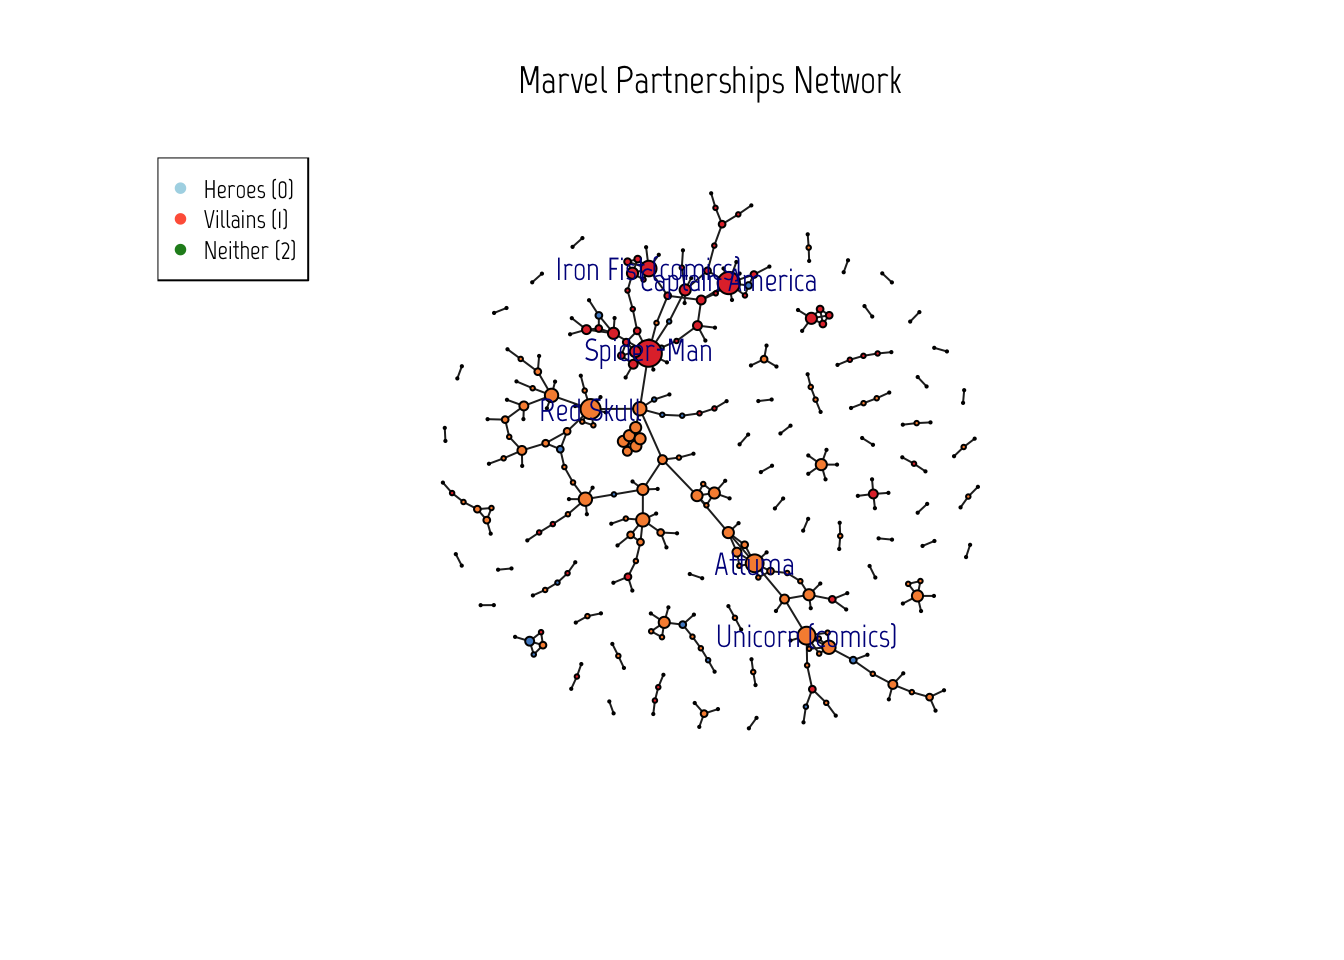
\includegraphics{Social_Network_1st_Assignment_files/figure-pdf/unnamed-chunk-10-1.pdf}

\begin{Shaded}
\begin{Highlighting}[]
\CommentTok{\# log{-}log}

\FunctionTok{plot}\NormalTok{(}\FunctionTok{table}\NormalTok{(degrees), }\AttributeTok{log =} \StringTok{"xy"}\NormalTok{, }\AttributeTok{main =} \StringTok{"Degree Distribution (Log{-}Log)"}\NormalTok{,}
     \AttributeTok{xlab =} \StringTok{"Degree"}\NormalTok{, }\AttributeTok{ylab =} \StringTok{"Frequency"}\NormalTok{, }\AttributeTok{pch =} \DecValTok{16}\NormalTok{, }\AttributeTok{col =} \StringTok{"\#0033A0"}\NormalTok{)}
\end{Highlighting}
\end{Shaded}

\includegraphics{Social_Network_1st_Assignment_files/figure-pdf/unnamed-chunk-10-2.pdf}

\begin{Shaded}
\begin{Highlighting}[]
\NormalTok{max\_degree }\OtherTok{\textless{}{-}} \FunctionTok{max}\NormalTok{(degrees)}
\end{Highlighting}
\end{Shaded}

\subsection{What is the clustering coefficient (transitivity) in the
network?}\label{what-is-the-clustering-coefficient-transitivity-in-the-network}

Transitivity measures how often nodes' neighbors are also connected. The
transitivity value of 0.2194149 indicates that the network is more
spread out than being tightly knit.

\begin{Shaded}
\begin{Highlighting}[]
\NormalTok{clustering\_coeff }\OtherTok{\textless{}{-}} \FunctionTok{transitivity}\NormalTok{(marvel\_network, }\AttributeTok{type =} \StringTok{"global"}\NormalTok{)}

\CommentTok{\#results}
\FunctionTok{cat}\NormalTok{(}\StringTok{"Clustering coefficient:"}\NormalTok{, clustering\_coeff, }\StringTok{"}\SpecialCharTok{\textbackslash{}n}\StringTok{"}\NormalTok{)}
\end{Highlighting}
\end{Shaded}

\begin{verbatim}
Clustering coefficient: 0.2194149 
\end{verbatim}

\subsection{What is the assortativity (degree) in the
network?}\label{what-is-the-assortativity-degree-in-the-network}

Assortativity measures if nodes with similar degrees connect (positive
value) or if high-degree nodes connect to low-degree ones (negative
value).

As explained earlier, we use `directed = FALSE' because our network is
bidirectional, meaning that a link (partnership) requires two parties.

The result (assortativity degree of -0.011047) shows that in the Marvel
network, characters with high numbers of partnerships slightly tend to
connect with those with fewer partnerships, but the effect is very weak
(because it is very close to 0), almost random.

\begin{Shaded}
\begin{Highlighting}[]
\NormalTok{assortativity\_degree }\OtherTok{\textless{}{-}} \FunctionTok{assortativity\_degree}\NormalTok{(marvel\_network, }\AttributeTok{directed =} \ConstantTok{FALSE}\NormalTok{)}

\CommentTok{\# result  }
\FunctionTok{cat}\NormalTok{(}\StringTok{"Assortativity (degree):"}\NormalTok{, assortativity\_degree, }\StringTok{"}\SpecialCharTok{\textbackslash{}n}\StringTok{"}\NormalTok{)}
\end{Highlighting}
\end{Shaded}

\begin{verbatim}
Assortativity (degree): -0.011047 
\end{verbatim}

Visually:

\begin{Shaded}
\begin{Highlighting}[]
\FunctionTok{V}\NormalTok{(marvel\_network)}\SpecialCharTok{$}\NormalTok{degree }\OtherTok{\textless{}{-}} \FunctionTok{degree}\NormalTok{(marvel\_network, }\AttributeTok{mode =} \StringTok{"all"}\NormalTok{)}

\CommentTok{\# Plot with igraph using a different layout}
\FunctionTok{plot}\NormalTok{(marvel\_network, }
     \AttributeTok{layout =} \FunctionTok{layout\_with\_kk}\NormalTok{(marvel\_network),  }\CommentTok{\# kamada{-}kawaii layout}
     \AttributeTok{vertex.size =} \FunctionTok{V}\NormalTok{(marvel\_network)}\SpecialCharTok{$}\NormalTok{degree }\SpecialCharTok{/} \DecValTok{2}\NormalTok{,}
     \AttributeTok{vertex.color =} \FunctionTok{colorRampPalette}\NormalTok{(}\FunctionTok{c}\NormalTok{(}\StringTok{"\#0033A0"}\NormalTok{,}
                                       \StringTok{"\#B40000"}\NormalTok{))(}\FunctionTok{max}\NormalTok{(}\FunctionTok{V}\NormalTok{(marvel\_network)}\SpecialCharTok{$}\NormalTok{degree) }\SpecialCharTok{+} \DecValTok{1}\NormalTok{)[}\FunctionTok{V}\NormalTok{(marvel\_network)}\SpecialCharTok{$}\NormalTok{degree }\SpecialCharTok{+} \DecValTok{1}\NormalTok{],}
     \AttributeTok{vertex.label =} \ConstantTok{NA}\NormalTok{,}
     \AttributeTok{edge.alpha =} \FloatTok{0.5}\NormalTok{,}
     \AttributeTok{main =} \StringTok{"Assortativity Visualization"}\NormalTok{)}
\end{Highlighting}
\end{Shaded}

\includegraphics{Social_Network_1st_Assignment_files/figure-pdf/marvel-assortativity-1.pdf}

\subsection{Using the Louvain method, does the network have a community
structure?}\label{using-the-louvain-method-does-the-network-have-a-community-structure}

Initially we wanted to check if there's a community structure with and
without edge weights. However, our network is not one that shows the
strength or times of occurrence of edges, rather, it only shows the
number of partnerships that existed at some point. That is why we
decided to assess the community structure with `weights = NULL'.

So, yes, the network exhibits a clear community structure, as shown in
the plot where nodes are grouped into distinct clusters with distinct
colors and labeled IDs, indicating that characters form close groups
with more internal connections than external ones, a hallmark of
community structure.

\begin{Shaded}
\begin{Highlighting}[]
\FunctionTok{set.seed}\NormalTok{(}\DecValTok{616}\NormalTok{)}
\NormalTok{comm\_without\_weights }\OtherTok{\textless{}{-}} \FunctionTok{cluster\_louvain}\NormalTok{(marvel\_network,}\AttributeTok{weights=}\ConstantTok{NULL}\NormalTok{)}

\FunctionTok{sizes}\NormalTok{(comm\_without\_weights)}
\end{Highlighting}
\end{Shaded}

\begin{verbatim}
Community sizes
 1  2  3  4  5  6  7  8  9 10 11 12 13 14 15 16 17 18 19 20 21 22 23 24 25 26 
 3  7  2  8  3 11  4  2 14  2  6  3  2 23  5 21 17 22 13  3  3  2  2  3  2  2 
27 28 29 30 31 32 33 34 35 36 37 38 39 40 41 42 43 44 45 46 47 48 49 50 51 52 
 3  2  6 23 15 25  4  5  2  4  2  4  2  2  2  6  2  2  3  5  4  3  2  2  2  2 
53 54 55 56 57 58 59 60 61 62 63 64 65 
 2  2  3  3  2  2  2  2  2  5  2  2  2 
\end{verbatim}

Plotting the community structure

\begin{Shaded}
\begin{Highlighting}[]
\FunctionTok{plot}\NormalTok{(comm\_without\_weights, marvel\_network)}
\end{Highlighting}
\end{Shaded}

\includegraphics{Social_Network_1st_Assignment_files/figure-pdf/marvel-network-plot4-1.pdf}

Let's check the community structure with weights just in case. Results
are pretty much the same. Does this most probably imply that the network
does not suit for a weighted assessment of community structure?

\begin{Shaded}
\begin{Highlighting}[]
\NormalTok{comm\_with\_weights }\OtherTok{\textless{}{-}} \FunctionTok{cluster\_louvain}\NormalTok{(marvel\_network,}
                                     \AttributeTok{weights =} \FunctionTok{E}\NormalTok{(marvel\_network)}\SpecialCharTok{$}\NormalTok{size)}
\FunctionTok{sizes}\NormalTok{(comm\_with\_weights)}
\end{Highlighting}
\end{Shaded}

\begin{verbatim}
Community sizes
 1  2  3  4  5  6  7  8  9 10 11 12 13 14 15 16 17 18 19 20 21 22 23 24 25 26 
 3  7  2  8  3 11  4  2 14  2  6  3  2 23  5 18 17 22 13  3  3  2  2  3  2  2 
27 28 29 30 31 32 33 34 35 36 37 38 39 40 41 42 43 44 45 46 47 48 49 50 51 52 
 3  2  6 23 15 19  4  5  9  2  4  2  4  2  2  2  6  2  2  3  5  4  3  2  2  2 
53 54 55 56 57 58 59 60 61 62 63 64 65 66 
 2  2  2  3  3  2  2  2  2  2  5  2  2  2 
\end{verbatim}

\begin{Shaded}
\begin{Highlighting}[]
\CommentTok{\# plotting}

\FunctionTok{plot}\NormalTok{(comm\_with\_weights, marvel\_network)}
\end{Highlighting}
\end{Shaded}

\includegraphics{Social_Network_1st_Assignment_files/figure-pdf/marvel-network-plot5-1.pdf}

\begin{center}\rule{0.5\linewidth}{0.5pt}\end{center}

\subsection{If so, what is its
modularity?}\label{if-so-what-is-its-modularity}

The modularity score of 0.9116242 indicates a very strong community
structure in the Marvel network, as values close to 1 suggest that the
Louvain method found highly distinct groups where characters are much
more connected within their communities than expected in a random
network.

This aligns with the visual clustering in our plot, confirming that the
network has well-defined, meaningful communities.

\begin{Shaded}
\begin{Highlighting}[]
\FunctionTok{set.seed}\NormalTok{(}\DecValTok{616}\NormalTok{)}
\FunctionTok{modularity}\NormalTok{(comm\_without\_weights)}
\end{Highlighting}
\end{Shaded}

\begin{verbatim}
[1] 0.9116242
\end{verbatim}

Below plot visualizes the network with communities from
comm\_without\_weights, using the Kamada-Kawai layout ll, coloring nodes
by community, and omitting vertex labels for clarity.

The Kamada-Kawai layout tries to put characters closer if they're
partners and further apart if they're not, making the plot and structure
easier to understand.

\begin{Shaded}
\begin{Highlighting}[]
\NormalTok{ll }\OtherTok{\textless{}{-}} \FunctionTok{layout.kamada.kawai}\NormalTok{(marvel\_network)}
\FunctionTok{plot}\NormalTok{(comm\_without\_weights,marvel\_network,}\AttributeTok{layout=}\NormalTok{ll,}\AttributeTok{vertex.label=}\StringTok{""}\NormalTok{)}
\end{Highlighting}
\end{Shaded}

\includegraphics{Social_Network_1st_Assignment_files/figure-pdf/marvel-network-plot6-1.pdf}

\subsection{Test that the clustering coefficient in the network cannot
be statistically explained by a configuration model in which the nodes
have the same degree distribution as the
original.}\label{test-that-the-clustering-coefficient-in-the-network-cannot-be-statistically-explained-by-a-configuration-model-in-which-the-nodes-have-the-same-degree-distribution-as-the-original.}

After generating a degree-preserving rewired version of the Marvel
network across 100 random times, we find that the clustering coefficient
drops from 0.219 (the original Marvel network clustering coefficient) to
0.006382979 (the mean of the simulated clusterings). The p-value of 0
feels fishy in the beginning, however, it only indicates that none of
the simulations were as high as or higher than the original one.

This significant decrease suggests that the clustering structure
observed in the real network is not explained by the degree distribution
alone. Instead, it reflects meaningful group structures, such as
narrative teams or recurring character associations in the Marvel
universe.

The original Marvel network has much higher clustering than its
degree-preserving random counterpart: characters that are connected to
the same person tend to be connected to each other --- suggesting
intentional grouping or narrative structure (such as teams like Avengers
or X-Men).

In the rewired version, where the number of connections for each
character is preserved but partners are randomized, that natural
tendency disappears.

\begin{Shaded}
\begin{Highlighting}[]
\FunctionTok{set.seed}\NormalTok{(}\DecValTok{616}\NormalTok{)}

\NormalTok{sim\_clustering }\OtherTok{\textless{}{-}} \FunctionTok{replicate}\NormalTok{(}\DecValTok{100}\NormalTok{, \{}
\NormalTok{  g\_rewired }\OtherTok{\textless{}{-}} \FunctionTok{rewire}\NormalTok{(marvel\_network,}
                      \AttributeTok{with =} \FunctionTok{keeping\_degseq}\NormalTok{(}\AttributeTok{niter =} \FunctionTok{ecount}\NormalTok{(marvel\_network) }\SpecialCharTok{*} \DecValTok{10}\NormalTok{))}
  \FunctionTok{transitivity}\NormalTok{(g\_rewired, }\AttributeTok{type =} \StringTok{"global"}\NormalTok{)}
\NormalTok{\})}

\NormalTok{observed\_clustering }\OtherTok{\textless{}{-}} \FunctionTok{transitivity}\NormalTok{(marvel\_network, }\AttributeTok{type =} \StringTok{"global"}\NormalTok{)}

\CommentTok{\# computing p{-}value, meaning the proportion of simulated clustering ≥ observed)}
\NormalTok{p\_val }\OtherTok{\textless{}{-}} \FunctionTok{mean}\NormalTok{(sim\_clustering }\SpecialCharTok{\textgreater{}=}\NormalTok{ observed\_clustering)}

\FunctionTok{cat}\NormalTok{(}\StringTok{"Observed clustering:"}\NormalTok{, observed\_clustering, }\StringTok{"}\SpecialCharTok{\textbackslash{}n}\StringTok{"}\NormalTok{)}
\end{Highlighting}
\end{Shaded}

\begin{verbatim}
Observed clustering: 0.2194149 
\end{verbatim}

\begin{Shaded}
\begin{Highlighting}[]
\FunctionTok{cat}\NormalTok{(}\StringTok{"Mean simulated clustering:"}\NormalTok{, }\FunctionTok{mean}\NormalTok{(sim\_clustering), }\StringTok{"}\SpecialCharTok{\textbackslash{}n}\StringTok{"}\NormalTok{)}
\end{Highlighting}
\end{Shaded}

\begin{verbatim}
Mean simulated clustering: 0.006382979 
\end{verbatim}

\begin{Shaded}
\begin{Highlighting}[]
\FunctionTok{cat}\NormalTok{(}\StringTok{"p{-}value:"}\NormalTok{, p\_val, }\StringTok{"}\SpecialCharTok{\textbackslash{}n}\StringTok{"}\NormalTok{)}
\end{Highlighting}
\end{Shaded}

\begin{verbatim}
p-value: 0 
\end{verbatim}

\subsubsection{Comparing the two
networks}\label{comparing-the-two-networks}

\begin{Shaded}
\begin{Highlighting}[]
\NormalTok{data }\OtherTok{\textless{}{-}} \FunctionTok{data.frame}\NormalTok{(}
  \AttributeTok{Network =} \FunctionTok{c}\NormalTok{(}\StringTok{"Original"}\NormalTok{, }\StringTok{"Simulated Mean"}\NormalTok{),}
  \AttributeTok{Clustering =} \FunctionTok{c}\NormalTok{(observed\_clustering, }\FunctionTok{mean}\NormalTok{(sim\_clustering))}
\NormalTok{)}

\FunctionTok{ggplot}\NormalTok{(data, }\FunctionTok{aes}\NormalTok{(}\AttributeTok{x =}\NormalTok{ Network, }\AttributeTok{y =}\NormalTok{ Clustering, }\AttributeTok{fill =}\NormalTok{ Network)) }\SpecialCharTok{+}
  \FunctionTok{geom\_col}\NormalTok{(}\AttributeTok{width =} \FloatTok{0.5}\NormalTok{) }\SpecialCharTok{+}
  \FunctionTok{geom\_text}\NormalTok{(}\FunctionTok{aes}\NormalTok{(}\AttributeTok{label =} \FunctionTok{round}\NormalTok{(Clustering, }\DecValTok{3}\NormalTok{)), }\AttributeTok{vjust =} \SpecialCharTok{{-}}\FloatTok{0.5}\NormalTok{) }\SpecialCharTok{+}
  \FunctionTok{scale\_fill\_manual}\NormalTok{(}\AttributeTok{values =} \FunctionTok{c}\NormalTok{(}\StringTok{"Original"} \OtherTok{=} \StringTok{"\#3C9A3F"}\NormalTok{,}
                               \StringTok{"Simulated Mean"} \OtherTok{=} \StringTok{"\#D6A400"}\NormalTok{)) }\SpecialCharTok{+}
  \FunctionTok{labs}\NormalTok{(}\AttributeTok{title =} \StringTok{"Clustering Coefficient: Observed vs. Simulated"}\NormalTok{,}
       \AttributeTok{y =} \StringTok{"Clustering Coefficient"}\NormalTok{) }\SpecialCharTok{+}
  \FunctionTok{theme\_minimal}\NormalTok{()}
\end{Highlighting}
\end{Shaded}

\includegraphics{Social_Network_1st_Assignment_files/figure-pdf/unnamed-chunk-16-1.pdf}

\subsection{Visualize the neighborhood of the node with the largest
centrality
(closeness).}\label{visualize-the-neighborhood-of-the-node-with-the-largest-centrality-closeness.}

igraph package has several ways to calculate centrality of nodes and
edges. Let's try them and see how the results differ.

\subsubsection{PageRank: calculates Google's PageRank for
vertices}\label{pagerank-calculates-googles-pagerank-for-vertices}

Below chunk calculates the PageRank scores for nodes in marvel\_network,
which measures node importance based on connections --- nodes with more
links from other important nodes get higher scores.

The results show Spider-Man, Captain America, Red Skull, Selene,
Unicorn, and Grim Reaper as the top 6, indicating they are the most
influential characters in the network, likely due to their connections
to other highly connected characters, such as Spider-Man and Captain
America linking to many key Avengers or Red Skull to major villains.

\begin{Shaded}
\begin{Highlighting}[]
\CommentTok{\# pageRank centrality computation}
\NormalTok{page\_rank\_marvel }\OtherTok{\textless{}{-}} \FunctionTok{page\_rank}\NormalTok{(marvel\_network)}

\CommentTok{\# top characters}

\NormalTok{top\_pr }\OtherTok{\textless{}{-}}\NormalTok{ page\_rank\_marvel}\SpecialCharTok{$}\NormalTok{vector }\SpecialCharTok{\%\textgreater{}\%} 
  \FunctionTok{sort}\NormalTok{(}\AttributeTok{decreasing =} \ConstantTok{TRUE}\NormalTok{) }\SpecialCharTok{\%\textgreater{}\%} \FunctionTok{head}\NormalTok{()}

\FunctionTok{data.frame}\NormalTok{(}
  \AttributeTok{character\_name =} \FunctionTok{V}\NormalTok{(marvel\_network)}\SpecialCharTok{$}\NormalTok{character\_name[}\FunctionTok{as.numeric}\NormalTok{(}\FunctionTok{names}\NormalTok{(top\_pr))],}
  \AttributeTok{page\_rank =}\NormalTok{ top\_pr}
\NormalTok{)}
\end{Highlighting}
\end{Shaded}

\begin{verbatim}
     character_name   page_rank
194      Spider-Man 0.010885939
302 Captain America 0.010575984
306       Red Skull 0.009778847
12           Selene 0.008108108
220         Unicorn 0.007716852
276     Grim Reaper 0.007562538
\end{verbatim}

\subsubsection{Closeness: distance (steps) to any other
vertex}\label{closeness-distance-steps-to-any-other-vertex}

Closeness calculates the closeness centrality for each node in the
network, measuring how close a node is to all others. Higher values mean
closer, fewer steps to reach others.

The results, with closeness of 1 for Silver Sable, U.S. Agent, Hercules,
Sabretooth, Mojo, and Trevor Fitzroy, indicate these characters have the
highest closeness, meaning they are in small, isolated components, where
they are directly connected to all others in their component, inflating
their scores. We consider that these characters have perfect centrality
scores because the closeness method assesses their local communities,
rather than the network as a whole.

\begin{Shaded}
\begin{Highlighting}[]
\CommentTok{\# closeness  computation}
\NormalTok{closeness\_marvel }\OtherTok{\textless{}{-}} \FunctionTok{closeness}\NormalTok{(marvel\_network)}

\CommentTok{\# to get the top characters}

\NormalTok{top\_closeness }\OtherTok{\textless{}{-}} \DecValTok{1}\SpecialCharTok{/}\NormalTok{closeness\_marvel }\SpecialCharTok{\%\textgreater{}\%} \FunctionTok{sort}\NormalTok{(}\AttributeTok{decreasing =} \ConstantTok{TRUE}\NormalTok{) }\SpecialCharTok{\%\textgreater{}\%} \FunctionTok{head}\NormalTok{()}
\FunctionTok{data.frame}\NormalTok{(}
  \AttributeTok{character\_name =} \FunctionTok{V}\NormalTok{(marvel\_network)}\SpecialCharTok{$}\NormalTok{character\_name[}\FunctionTok{as.numeric}\NormalTok{(}\FunctionTok{names}\NormalTok{(top\_closeness))],}
  \AttributeTok{inverse\_closeness =}\NormalTok{ top\_closeness}
\NormalTok{)}
\end{Highlighting}
\end{Shaded}

\begin{verbatim}
   character_name inverse_closeness
3    Silver Sable                 1
9      U.S. Agent                 1
11       Hercules                 1
14     Sabretooth                 1
28           Mojo                 1
29 Trevor Fitzroy                 1
\end{verbatim}

Betweenness method looks into the number of shortest paths going through
an edge.

The results show Venom, Doctor Doom, Spider-Man, Puppet Master, Krang,
and Attuma as the top six characters, meaning they are key bridges in
the network, frequently connecting other characters.

\begin{Shaded}
\begin{Highlighting}[]
\CommentTok{\# betweenness centrality computation}
\NormalTok{betweenness\_marvel }\OtherTok{\textless{}{-}} \FunctionTok{betweenness}\NormalTok{(marvel\_network)}

\CommentTok{\# top characters}
\NormalTok{top\_betweenness }\OtherTok{\textless{}{-}}\NormalTok{ betweenness\_marvel }\SpecialCharTok{\%\textgreater{}\%} \FunctionTok{sort}\NormalTok{(}\AttributeTok{decreasing =} \ConstantTok{TRUE}\NormalTok{) }\SpecialCharTok{\%\textgreater{}\%} \FunctionTok{head}\NormalTok{()}
\FunctionTok{data.frame}\NormalTok{(}
  \AttributeTok{character\_name =} \FunctionTok{V}\NormalTok{(marvel\_network)}\SpecialCharTok{$}\NormalTok{character\_name[}\FunctionTok{as.numeric}\NormalTok{(}\FunctionTok{names}\NormalTok{(top\_betweenness))],}
  \AttributeTok{betweenness =}\NormalTok{ top\_betweenness}
\NormalTok{)}
\end{Highlighting}
\end{Shaded}

\begin{verbatim}
    character_name betweenness
10           Venom    10704.50
182    Doctor Doom     9108.00
194     Spider-Man     7904.25
330  Puppet Master     6461.50
123          Krang     5739.00
239         Attuma     5361.50
\end{verbatim}

\paragraph{Harmonic Centrality}\label{harmonic-centrality}

As suggested, we decided to calculate the harmonic centrality for our
characters in the network. We did so using the harmonic\_centrality
function from the igraph package. Harmonic centrality is a measure that
gives higher scores to nodes that are closer to other nodes in the
network. It is particularly useful in networks where shortest path
calculations are important.

Below are the top 6 characters by harmonic centrality scores.

\begin{Shaded}
\begin{Highlighting}[]
\FunctionTok{library}\NormalTok{(tidygraph)}
\CommentTok{\# harmonic centrality}
\NormalTok{cent\_harmonic }\OtherTok{\textless{}{-}} \FunctionTok{harmonic\_centrality}\NormalTok{(marvel\_network)}

\NormalTok{centrality\_df }\OtherTok{\textless{}{-}} \FunctionTok{data.frame}\NormalTok{(}
  \AttributeTok{character\_name =} \FunctionTok{V}\NormalTok{(marvel\_network)}\SpecialCharTok{$}\NormalTok{character\_name,}
  \AttributeTok{harmonic\_centrality =} \FunctionTok{harmonic\_centrality}\NormalTok{(marvel\_network)}
\NormalTok{)}

\NormalTok{top\_harmonic }\OtherTok{\textless{}{-}}\NormalTok{ centrality\_df[}\FunctionTok{order}\NormalTok{(}\SpecialCharTok{{-}}\NormalTok{centrality\_df}\SpecialCharTok{$}\NormalTok{harmonic\_centrality), ][}\DecValTok{1}\SpecialCharTok{:}\DecValTok{6}\NormalTok{, ]}
\FunctionTok{print}\NormalTok{(top\_harmonic)}
\end{Highlighting}
\end{Shaded}

\begin{verbatim}
    character_name harmonic_centrality
10           Venom            51.50792
194     Spider-Man            51.45044
306      Red Skull            47.24529
182    Doctor Doom            46.72146
330  Puppet Master            42.20920
71     Enchantress            41.90316
\end{verbatim}

We can use a scatter plot or a bar plot to visualize the harmonic
centrality of nodes. We used a scatter plot with ggplot2 to compare
harmonic centrality with other centrality measures.

This plot compares harmonic centrality with closeness centrality, with
nodes colored by their PageRank. This allows us to see how these
centrality measures relate to each other. Nodes with high harmonic
centrality and closeness centrality are likely important connectors in
the network.

\begin{Shaded}
\begin{Highlighting}[]
\NormalTok{centrality\_df }\OtherTok{\textless{}{-}} \FunctionTok{data.frame}\NormalTok{(}
  \AttributeTok{character\_name =} \FunctionTok{V}\NormalTok{(marvel\_network)}\SpecialCharTok{$}\NormalTok{name,}
  \AttributeTok{harmonic\_centrality =} \FunctionTok{harmonic\_centrality}\NormalTok{(marvel\_network),}
  \AttributeTok{closeness =} \FunctionTok{closeness}\NormalTok{(marvel\_network),}
  \AttributeTok{page\_rank =} \FunctionTok{page\_rank}\NormalTok{(marvel\_network)}\SpecialCharTok{$}\NormalTok{vector}
\NormalTok{)}


\CommentTok{\# harmonic centrality vs. other centrality measures}
\FunctionTok{ggplot}\NormalTok{(centrality\_df, }\FunctionTok{aes}\NormalTok{(}\AttributeTok{x =}\NormalTok{ harmonic\_centrality,}
                          \AttributeTok{y =}\NormalTok{ closeness, }\AttributeTok{color =}\NormalTok{ page\_rank)) }\SpecialCharTok{+}
  \FunctionTok{geom\_point}\NormalTok{(}\AttributeTok{alpha =} \FloatTok{0.6}\NormalTok{, }\AttributeTok{size =} \DecValTok{3}\NormalTok{) }\SpecialCharTok{+}
  \FunctionTok{labs}\NormalTok{(}\AttributeTok{title =} \StringTok{"Harmonic Centrality vs. Closeness Centrality"}\NormalTok{,}
       \AttributeTok{x =} \StringTok{"Harmonic Centrality"}\NormalTok{,}
       \AttributeTok{y =} \StringTok{"Closeness Centrality"}\NormalTok{,}
       \AttributeTok{color =} \StringTok{"PageRank"}\NormalTok{) }\SpecialCharTok{+}
  \FunctionTok{theme\_minimal}\NormalTok{() }\SpecialCharTok{+}
  \FunctionTok{theme}\NormalTok{(}\AttributeTok{plot.title =} \FunctionTok{element\_text}\NormalTok{(}\AttributeTok{family =} \StringTok{"Marvel"}\NormalTok{, }\AttributeTok{size =} \DecValTok{16}\NormalTok{))}
\end{Highlighting}
\end{Shaded}

\includegraphics{Social_Network_1st_Assignment_files/figure-pdf/unnamed-chunk-21-1.pdf}

Alternatively, we can visualize the top nodes by harmonic centrality
through a bar plot. This plot shows the top 10 characters by harmonic
centrality, allowing us to easily identify the most central nodes.

\begin{Shaded}
\begin{Highlighting}[]
\CommentTok{\# top nodes by harmonic centrality}
\NormalTok{top\_harmonic\_plot }\OtherTok{\textless{}{-}}\NormalTok{ centrality\_df[}\FunctionTok{order}\NormalTok{(}\SpecialCharTok{{-}}\NormalTok{centrality\_df}\SpecialCharTok{$}\NormalTok{harmonic\_centrality), ][}\DecValTok{1}\SpecialCharTok{:}\DecValTok{10}\NormalTok{, ]}

\FunctionTok{ggplot}\NormalTok{(top\_harmonic\_plot, }\FunctionTok{aes}\NormalTok{(}\AttributeTok{x =} \FunctionTok{reorder}\NormalTok{(character\_name, harmonic\_centrality),}
                              \AttributeTok{y =}\NormalTok{ harmonic\_centrality)) }\SpecialCharTok{+}
  \FunctionTok{geom\_bar}\NormalTok{(}\AttributeTok{stat =} \StringTok{"identity"}\NormalTok{, }\AttributeTok{fill =} \StringTok{"\#B40000"}\NormalTok{) }\SpecialCharTok{+}
  \FunctionTok{coord\_flip}\NormalTok{() }\SpecialCharTok{+}
  \FunctionTok{labs}\NormalTok{(}\AttributeTok{title =} \StringTok{"Top 10 Characters by Harmonic Centrality"}\NormalTok{,}
       \AttributeTok{x =} \StringTok{"Character Name"}\NormalTok{,}
       \AttributeTok{y =} \StringTok{"Harmonic Centrality"}\NormalTok{) }\SpecialCharTok{+}
  \FunctionTok{theme\_minimal}\NormalTok{() }\SpecialCharTok{+}
  \FunctionTok{theme}\NormalTok{(}\AttributeTok{plot.title =} \FunctionTok{element\_text}\NormalTok{(}\AttributeTok{family =} \StringTok{"Marvel"}\NormalTok{, }\AttributeTok{size =} \DecValTok{16}\NormalTok{))}
\end{Highlighting}
\end{Shaded}

\includegraphics{Social_Network_1st_Assignment_files/figure-pdf/unnamed-chunk-22-1.pdf}

\subsubsection{The neighbourhood of the most central node -
VENOM}\label{the-neighbourhood-of-the-most-central-node---venom}

According to our harmonic centrality measure, Venom is the most central
character in the entire Marvel network. Indeed, if we zoom in even on
his 1-step neighbourhood, we see that he formed partnerships with
different type of characters such as heroes (Spider-Man), villains (Red
Skull, Doctor Doom, Carnage), and neutral characters (Magneto, Eddie
Brock).

Note that Eddie Brock is the human form of Venom, who is considered to
be (or to have become) a neutral/antihero character.

\begin{Shaded}
\begin{Highlighting}[]
\CommentTok{\# venom\textquotesingle{}s id}
\NormalTok{venom\_id }\OtherTok{\textless{}{-}}\NormalTok{ marvel\_nodes}\SpecialCharTok{$}\NormalTok{id[marvel\_nodes}\SpecialCharTok{$}\NormalTok{character\_name }\SpecialCharTok{==} \StringTok{"Venom"}\NormalTok{]}
\FunctionTok{print}\NormalTok{(venom\_id)}
\end{Highlighting}
\end{Shaded}

\begin{verbatim}
[1] 10
\end{verbatim}

\begin{Shaded}
\begin{Highlighting}[]
\CommentTok{\# detecting the node}
\NormalTok{venom\_node }\OtherTok{\textless{}{-}} \FunctionTok{which}\NormalTok{(}\FunctionTok{V}\NormalTok{(marvel\_network)}\SpecialCharTok{$}\NormalTok{name }\SpecialCharTok{==} \FunctionTok{as.character}\NormalTok{(venom\_id))}

\CommentTok{\# venom\textquotesingle{}s neighbourhood}
\NormalTok{venom\_neighborhood }\OtherTok{\textless{}{-}} \FunctionTok{ego}\NormalTok{(marvel\_network, }\AttributeTok{order =} \DecValTok{1}\NormalTok{, }\AttributeTok{nodes =}\NormalTok{ venom\_node,}
                          \AttributeTok{mode =} \StringTok{"all"}\NormalTok{)[[}\DecValTok{1}\NormalTok{]]}

\CommentTok{\# venom\textquotesingle{}s subgraph}
\NormalTok{venom\_subgraph }\OtherTok{\textless{}{-}} \FunctionTok{induced\_subgraph}\NormalTok{(marvel\_network, venom\_neighborhood)}

\CommentTok{\# ensuring nodes are represented with names}
\FunctionTok{V}\NormalTok{(venom\_subgraph)}\SpecialCharTok{$}\NormalTok{label }\OtherTok{\textless{}{-}} 
\NormalTok{  marvel\_nodes}\SpecialCharTok{$}\NormalTok{character\_name[}\FunctionTok{match}\NormalTok{(}\FunctionTok{V}\NormalTok{(venom\_subgraph)}\SpecialCharTok{$}\NormalTok{name, marvel\_nodes}\SpecialCharTok{$}\NormalTok{id)]}

\NormalTok{node\_groups }\OtherTok{\textless{}{-}}\NormalTok{ marvel\_nodes}\SpecialCharTok{$}\NormalTok{group[}\FunctionTok{match}\NormalTok{(}\FunctionTok{V}\NormalTok{(venom\_subgraph)}\SpecialCharTok{$}\NormalTok{name, marvel\_nodes}\SpecialCharTok{$}\NormalTok{id)]}

\NormalTok{node\_groups }\OtherTok{\textless{}{-}} \FunctionTok{as.numeric}\NormalTok{(node\_groups)}

\CommentTok{\#  group colors}
\NormalTok{group\_colors }\OtherTok{\textless{}{-}} \FunctionTok{c}\NormalTok{(}\StringTok{"0"} \OtherTok{=} \StringTok{"\#B40000"}\NormalTok{, }\StringTok{"1"} \OtherTok{=} \StringTok{"\#0033A0"}\NormalTok{, }\StringTok{"2"} \OtherTok{=} \StringTok{"\#3C9A3F"}\NormalTok{)}

\CommentTok{\# group values to colors}
\NormalTok{vertex\_colors }\OtherTok{\textless{}{-}}\NormalTok{ group\_colors[}\FunctionTok{as.character}\NormalTok{(node\_groups)]}

\CommentTok{\# plotting venom\textquotesingle{}s neighbourhood}
\FunctionTok{plot}\NormalTok{(venom\_subgraph,}
     \AttributeTok{layout =} \FunctionTok{layout\_with\_fr}\NormalTok{(venom\_subgraph), }
     \AttributeTok{vertex.label =} \FunctionTok{V}\NormalTok{(venom\_subgraph)}\SpecialCharTok{$}\NormalTok{label,}
     \AttributeTok{vertex.label.cex =} \FloatTok{0.8}\NormalTok{,}
     \AttributeTok{vertex.label.dist =} \FloatTok{1.2}\NormalTok{,}
     \AttributeTok{vertex.label.degree =}\NormalTok{ pi}\SpecialCharTok{/}\DecValTok{4}\NormalTok{,}
     \AttributeTok{vertex.color =}\NormalTok{ vertex\_colors,}
     \AttributeTok{vertex.size =} \DecValTok{12}\NormalTok{,}
     \AttributeTok{main =} \StringTok{"Venom\textquotesingle{}s Neighborhood"}\NormalTok{,}
     \AttributeTok{margin =} \SpecialCharTok{{-}}\FloatTok{0.05}\NormalTok{)}
\end{Highlighting}
\end{Shaded}

\includegraphics{Social_Network_1st_Assignment_files/figure-pdf/unnamed-chunk-23-1.pdf}

\paragraph{Comparison}\label{comparison}

To visually support our choices regarding the different centrality
measures, we wanted to create a plot to highlight how each measure ranks
the characters in the network.

This visualization helped us gain a comprehensive understanding of how
different centrality measures rank the characters in our network and how
these measures relate to each other.

A bar plot can be used to compare the rankings of characters across
different centrality measures. This can help identify which characters
are most central according to each measure.

Although some of the labels are not read properly, we can, by looking at
the distributions, say that betweenness method yields confusing results
by attributing no centrality to most characters whereas closeness method
detects most characters as having a centrality score of 1 (which is the
perfect score). This is due to the fact that closeness method sometimes
assesses characters based on their local communities in the network,
rather than the network as a whole, therefore spotting perfect
centrality.

Harmonic centrality and PageRank methods seem to provide more robust
results, assigning a range of centrality scores across characters. We,
upon the suggestion of the Professor, decided earlier to use harmonic
centrality to answer the question of most central node and its
neighbourhood.

\begin{Shaded}
\begin{Highlighting}[]
\NormalTok{centrality\_df}\SpecialCharTok{$}\NormalTok{betweenness }\OtherTok{\textless{}{-}} \FunctionTok{betweenness}\NormalTok{(marvel\_network)}

\CommentTok{\# adjusting the data for plotting}
\NormalTok{centrality\_long }\OtherTok{\textless{}{-}} \FunctionTok{pivot\_longer}\NormalTok{(centrality\_df,}
                                \AttributeTok{cols =} \FunctionTok{c}\NormalTok{(}\StringTok{"betweenness"}\NormalTok{, }\StringTok{"page\_rank"}\NormalTok{, }
                                         \StringTok{"closeness"}\NormalTok{,}
                                         \StringTok{"harmonic\_centrality"}\NormalTok{),}
                                \AttributeTok{names\_to =} \StringTok{"measure"}\NormalTok{, }\AttributeTok{values\_to =} \StringTok{"score"}\NormalTok{)}

\CommentTok{\# plot}
\FunctionTok{ggplot}\NormalTok{(centrality\_long, }\FunctionTok{aes}\NormalTok{(}\AttributeTok{x =} \FunctionTok{reorder}\NormalTok{(character\_name, score),}
                            \AttributeTok{y =}\NormalTok{ score, }\AttributeTok{fill =}\NormalTok{ measure)) }\SpecialCharTok{+}
  \FunctionTok{geom\_bar}\NormalTok{(}\AttributeTok{stat =} \StringTok{"identity"}\NormalTok{, }\AttributeTok{position =} \StringTok{"dodge"}\NormalTok{) }\SpecialCharTok{+}
  \FunctionTok{facet\_wrap}\NormalTok{(}\SpecialCharTok{\textasciitilde{}}\NormalTok{ measure, }\AttributeTok{scales =} \StringTok{"free"}\NormalTok{) }\SpecialCharTok{+}
  \FunctionTok{labs}\NormalTok{(}\AttributeTok{title =} \StringTok{"Centrality Measures Comparison"}\NormalTok{, }\AttributeTok{x =} \StringTok{"Character"}\NormalTok{,}
       \AttributeTok{y =} \StringTok{"Score"}\NormalTok{) }\SpecialCharTok{+}
  \FunctionTok{theme\_minimal}\NormalTok{() }\SpecialCharTok{+}
  \FunctionTok{theme}\NormalTok{(}\AttributeTok{axis.text.x =} \FunctionTok{element\_text}\NormalTok{(}\AttributeTok{angle =} \DecValTok{45}\NormalTok{, }\AttributeTok{hjust =} \DecValTok{1}\NormalTok{))}
\end{Highlighting}
\end{Shaded}

\includegraphics{Social_Network_1st_Assignment_files/figure-pdf/unnamed-chunk-24-1.pdf}




\end{document}
